\section{Aufbau der Lösung}\label{sec:01_02_aufbauLoesung}
Das Projekt zur Entwicklung eines graphbasierten Informationssystem für die Analyse sozialer Interaktionen im Deutschen Bundestag, welches \glqq Sentiments Of Bundestag\grqq{} genannt wurde, besteht, wie bereits erwähnt, aus sieben Teilprojekten. Im folgenden Abschnitt wird grob auf die Thematiken der einzelnen Gruppen eingegangen.

\begin{figure}[H]
    \centering
    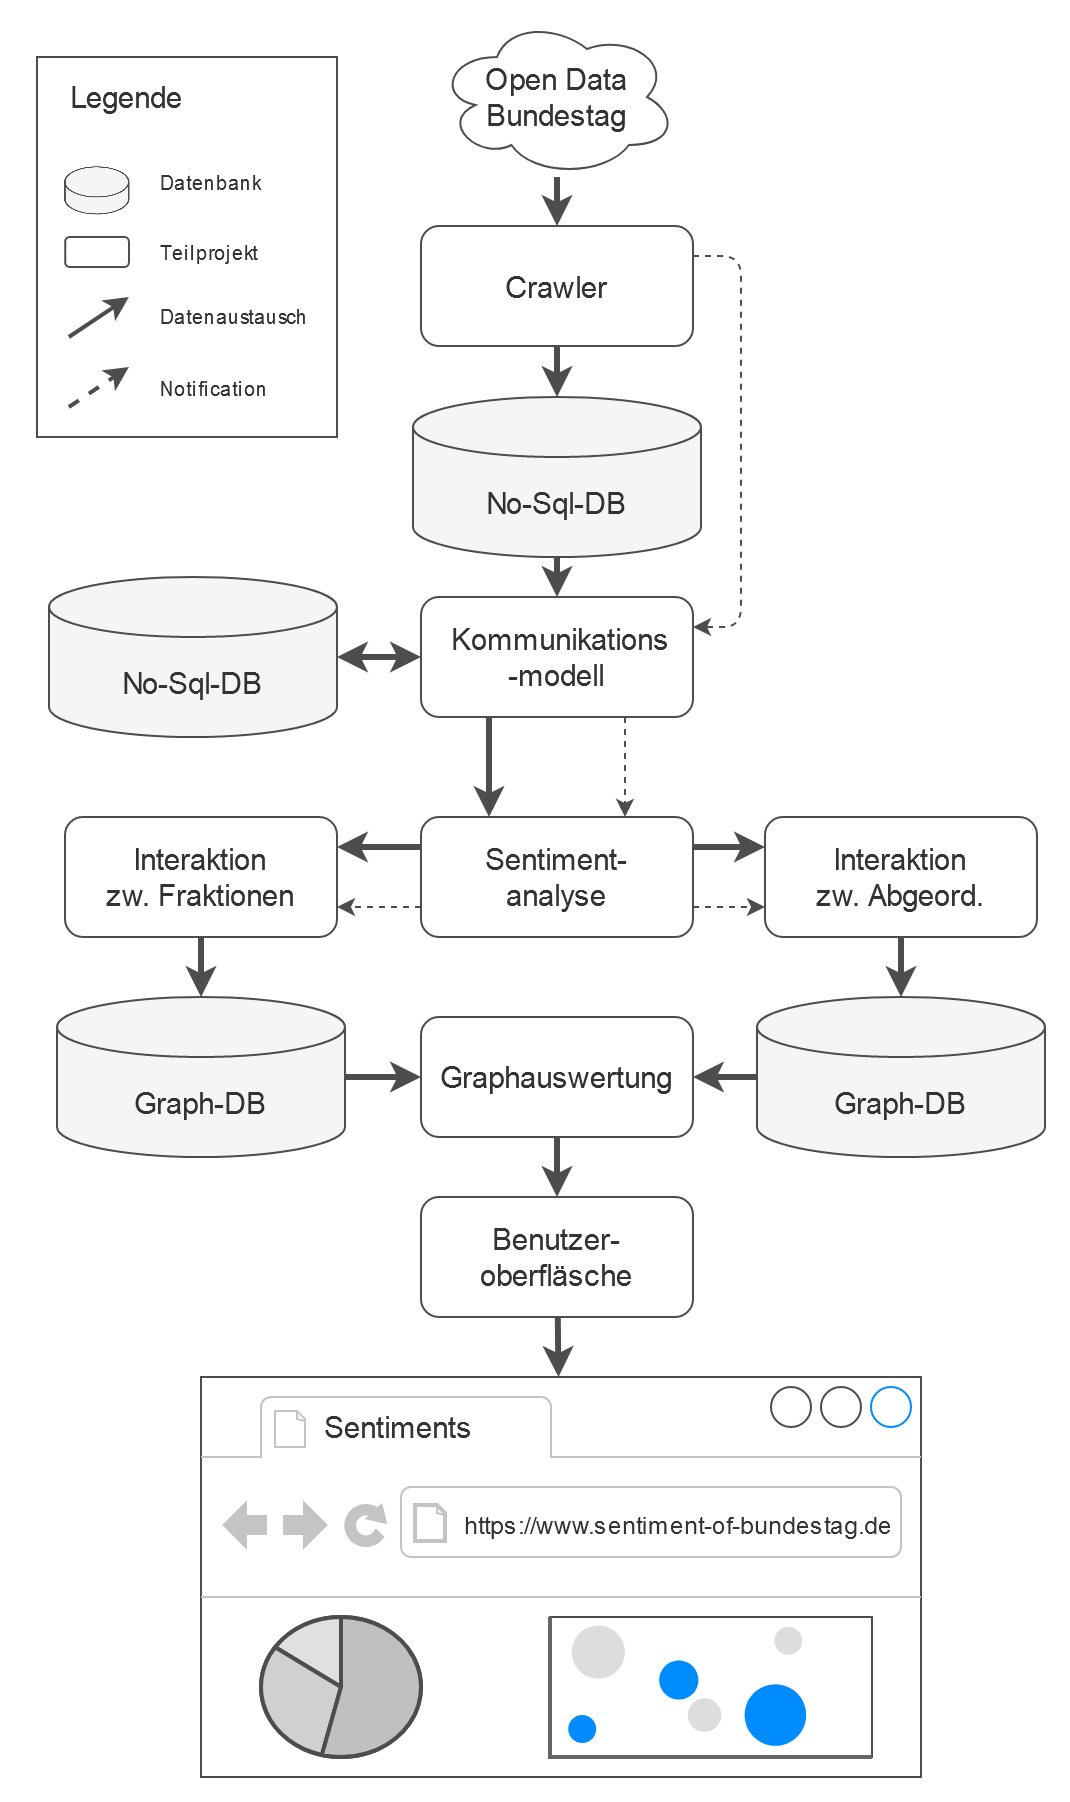
\includegraphics[width=\textwidth]{images/01-Einleitung/SentimentOfBundestag.png}
    \caption{Aufbau der Lösung}
    \label{fig:aufbauderLösungSOB}
\end{figure}

Die in \autoref{fig:aufbauderLösungSOB} dargestellten Teilprojekte sind hier nun detaillierter aufgelistet:
\begin{itemize}
    \item \textbf{Crawler}: Scannt regelmäßig die Open Data Webseite des Bundestags, sucht, parst und speichern neue Protokollen sowie Stammdaten der Abgeordneten in seiner No-Sql-Datenbank. Ziel ist es hier sicherzustellen, das die DB immer auf dem neusten Stand bleibt
    \item \textbf{Kommunikationsmodell}: Analysiert und erstellt aus den
      Protokollen von Gruppe 1 ein Kommunikationsmodell, welches die möglichen
      Interaktionen im Bundestag abbildet
    \item \textbf{Sentiment-Analyse}: Errechnet die Stimmung der von Gruppe 2 identifizierten Interaktionen und stellt Daten für Gruppe 3 und 4 bereit
    \item \textbf{Interaktion zwischen Abgeordneten}: Aus dem Kommunikationsmodell von Gruppe 2 und die Stimmungsanalyse von Gruppe 3 werden hier Interaktionen zwischen einzelnen Personen (Abgeordneten, Präsident, Gäste, etc.) identifiziert. Erstellt wird wird daraus ein gewichteter Sentiment-Graph zwischen Abgeordneten mit positiven/negativen Gewichtungen
    \item \textbf{Interaktion zwischen Fraktionen}: Aus dem Kommunikationsmodell von Gruppe 2 und den Sentiment-Graph zwischen Personen von Gruppe 4 werden hier Interaktionen zwischen Gruppen von Personen analysiert und in einen Sentiment-Graph zwischen Parteien. Der besteht aus einer Aggregation der Abgeordnetensentiments zu gewichteten Sentiment-Graph der Parteien (Fraktionen, Gruppen, etc.)
    \item \textbf{Graphauswertung}: Die Sentiment-Graphen von den Gruppen 4 und 5 werden hier anhand verschiedener Auswertungsmethoden analysiert und die Ergebnisse davon der nächsten Gruppe (Benutzeroberfläche) zur Verfügung gestellt
    \item \textbf{Benutzeroberfläche}: Ziel ist hier die Realisierung einer interaktiven Benutzeroberfläche zur Darstellung der Ergebnisse
\end{itemize}

Die einzelnen Teilprojekte werden in den nächsten Kapiteln von den jeweiligen Gruppenmitgliedern genauer erläutert.
